\tikzset{every picture/.style={line width=0.75pt}} %set default line width to 0.75pt        

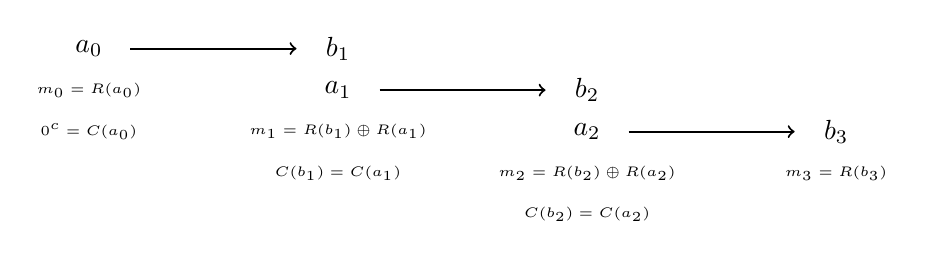
\begin{tikzpicture}[x=0.75pt,y=0.75pt,yscale=-1,xscale=1]
%uncomment if require: \path (0,300); %set diagram left start at 0, and has height of 300

%Straight Lines [id:da8110716189627085] 
\draw  [->]  (70,20) -- (150,20) ;
%Straight Lines [id:da7276012637365663] 
\draw  [->]  (190,40) -- (270,40) ;
%Straight Lines [id:da8434556424917563] 
\draw  [->]  (310,60) -- (390,60) ;

% Text Node
\draw (50.02,20) node    {$\mathpzc{a}_{0}$};
% Text Node
\draw (170,20) node    {$\mathpzc{b}_{1}$};
% Text Node
\draw (170,40) node    {$\mathpzc{a}_{1}$};
% Text Node
\draw (290,40) node    {$\mathpzc{b}_{2}$};
% Text Node
\draw (290,60) node    {$\mathpzc{a}_{2}$};
% Text Node
\draw (410,60) node    {$\mathpzc{b}_{3}$};
% Text Node
\draw (50,40) node  [font=\tiny]  {$m_{0}=R(\mathpzc{a}_{0})$};
% Text Node
\draw (50,60) node  [font=\tiny]  {$0^{c}=C(\mathpzc{a}_{0})$};
% Text Node
\draw (170,60) node  [font=\tiny]  {$m_{1}=R(\mathpzc{b}_{1}) \oplus R(\mathpzc{a}_{1})$};
% Text Node
\draw (170,80) node  [font=\tiny]  {$C(\mathpzc{b}_{1})=C(\mathpzc{a}_{1})$};
% Text Node
\draw (290,80) node  [font=\tiny]  {$m_{2}=R(\mathpzc{b}_{2}) \oplus R(\mathpzc{a}_{2})$};
% Text Node
\draw (290,100) node  [font=\tiny]  {$C(\mathpzc{b}_{2})=C(\mathpzc{a}_{2})$};
% Text Node
\draw (410,80) node  [font=\tiny]  {$m_{3}=R(\mathpzc{b}_{3})$};


\end{tikzpicture}